% Options for packages loaded elsewhere
\PassOptionsToPackage{unicode}{hyperref}
\PassOptionsToPackage{hyphens}{url}
\PassOptionsToPackage{dvipsnames,svgnames,x11names}{xcolor}
\documentclass[
  10pt,
]{article}
\usepackage{xcolor}
\usepackage[margin=2.0cm]{geometry}
\usepackage{amsmath,amssymb}
\setcounter{secnumdepth}{-\maxdimen} % remove section numbering
\usepackage{iftex}
\ifPDFTeX
  \usepackage[T1]{fontenc}
  \usepackage[utf8]{inputenc}
  \usepackage{textcomp} % provide euro and other symbols
\else % if luatex or xetex
  \usepackage{unicode-math} % this also loads fontspec
  \defaultfontfeatures{Scale=MatchLowercase}
  \defaultfontfeatures[\rmfamily]{Ligatures=TeX,Scale=1}
\fi
\usepackage{lmodern}
\ifPDFTeX\else
  % xetex/luatex font selection
\fi
% Use upquote if available, for straight quotes in verbatim environments
\IfFileExists{upquote.sty}{\usepackage{upquote}}{}
\IfFileExists{microtype.sty}{% use microtype if available
  \usepackage[]{microtype}
  \UseMicrotypeSet[protrusion]{basicmath} % disable protrusion for tt fonts
}{}
\makeatletter
\@ifundefined{KOMAClassName}{% if non-KOMA class
  \IfFileExists{parskip.sty}{%
    \usepackage{parskip}
  }{% else
    \setlength{\parindent}{0pt}
    \setlength{\parskip}{6pt plus 2pt minus 1pt}}
}{% if KOMA class
  \KOMAoptions{parskip=half}}
\makeatother
\usepackage{color}
\usepackage{fancyvrb}
\newcommand{\VerbBar}{|}
\newcommand{\VERB}{\Verb[commandchars=\\\{\}]}
\DefineVerbatimEnvironment{Highlighting}{Verbatim}{commandchars=\\\{\}}
% Add ',fontsize=\small' for more characters per line
\newenvironment{Shaded}{}{}
\newcommand{\AlertTok}[1]{\textcolor[rgb]{1.00,0.00,0.00}{\textbf{#1}}}
\newcommand{\AnnotationTok}[1]{\textcolor[rgb]{0.38,0.63,0.69}{\textbf{\textit{#1}}}}
\newcommand{\AttributeTok}[1]{\textcolor[rgb]{0.49,0.56,0.16}{#1}}
\newcommand{\BaseNTok}[1]{\textcolor[rgb]{0.25,0.63,0.44}{#1}}
\newcommand{\BuiltInTok}[1]{\textcolor[rgb]{0.00,0.50,0.00}{#1}}
\newcommand{\CharTok}[1]{\textcolor[rgb]{0.25,0.44,0.63}{#1}}
\newcommand{\CommentTok}[1]{\textcolor[rgb]{0.38,0.63,0.69}{\textit{#1}}}
\newcommand{\CommentVarTok}[1]{\textcolor[rgb]{0.38,0.63,0.69}{\textbf{\textit{#1}}}}
\newcommand{\ConstantTok}[1]{\textcolor[rgb]{0.53,0.00,0.00}{#1}}
\newcommand{\ControlFlowTok}[1]{\textcolor[rgb]{0.00,0.44,0.13}{\textbf{#1}}}
\newcommand{\DataTypeTok}[1]{\textcolor[rgb]{0.56,0.13,0.00}{#1}}
\newcommand{\DecValTok}[1]{\textcolor[rgb]{0.25,0.63,0.44}{#1}}
\newcommand{\DocumentationTok}[1]{\textcolor[rgb]{0.73,0.13,0.13}{\textit{#1}}}
\newcommand{\ErrorTok}[1]{\textcolor[rgb]{1.00,0.00,0.00}{\textbf{#1}}}
\newcommand{\ExtensionTok}[1]{#1}
\newcommand{\FloatTok}[1]{\textcolor[rgb]{0.25,0.63,0.44}{#1}}
\newcommand{\FunctionTok}[1]{\textcolor[rgb]{0.02,0.16,0.49}{#1}}
\newcommand{\ImportTok}[1]{\textcolor[rgb]{0.00,0.50,0.00}{\textbf{#1}}}
\newcommand{\InformationTok}[1]{\textcolor[rgb]{0.38,0.63,0.69}{\textbf{\textit{#1}}}}
\newcommand{\KeywordTok}[1]{\textcolor[rgb]{0.00,0.44,0.13}{\textbf{#1}}}
\newcommand{\NormalTok}[1]{#1}
\newcommand{\OperatorTok}[1]{\textcolor[rgb]{0.40,0.40,0.40}{#1}}
\newcommand{\OtherTok}[1]{\textcolor[rgb]{0.00,0.44,0.13}{#1}}
\newcommand{\PreprocessorTok}[1]{\textcolor[rgb]{0.74,0.48,0.00}{#1}}
\newcommand{\RegionMarkerTok}[1]{#1}
\newcommand{\SpecialCharTok}[1]{\textcolor[rgb]{0.25,0.44,0.63}{#1}}
\newcommand{\SpecialStringTok}[1]{\textcolor[rgb]{0.73,0.40,0.53}{#1}}
\newcommand{\StringTok}[1]{\textcolor[rgb]{0.25,0.44,0.63}{#1}}
\newcommand{\VariableTok}[1]{\textcolor[rgb]{0.10,0.09,0.49}{#1}}
\newcommand{\VerbatimStringTok}[1]{\textcolor[rgb]{0.25,0.44,0.63}{#1}}
\newcommand{\WarningTok}[1]{\textcolor[rgb]{0.38,0.63,0.69}{\textbf{\textit{#1}}}}
\usepackage{longtable,booktabs,array}
\usepackage{caption}
\captionsetup[table]{skip=6pt}
\newcounter{none} % for unnumbered tables
\usepackage{calc} % for calculating minipage widths
% Correct order of tables after \paragraph or \subparagraph
\usepackage{etoolbox}
\makeatletter
\patchcmd\longtable{\par}{\if@noskipsec\mbox{}\fi\par}{}{}
\makeatother
% Allow footnotes in longtable head/foot
\IfFileExists{footnotehyper.sty}{\usepackage{footnotehyper}}{\usepackage{footnote}}
\makesavenoteenv{longtable}
\usepackage{graphicx}
\makeatletter
\newsavebox\pandoc@box
\newcommand*\pandocbounded[1]{% scales image to fit in text height/width
  \sbox\pandoc@box{#1}%
  \Gscale@div\@tempa{\textheight}{\dimexpr\ht\pandoc@box+\dp\pandoc@box\relax}%
  \Gscale@div\@tempb{\linewidth}{\wd\pandoc@box}%
  \ifdim\@tempb\p@<\@tempa\p@\let\@tempa\@tempb\fi% select the smaller of both
  \ifdim\@tempa\p@<\p@\scalebox{\@tempa}{\usebox\pandoc@box}%
  \else\usebox{\pandoc@box}%
  \fi%
}
% Set default figure placement to htbp
\def\fps@figure{htbp}
\makeatother
\setlength{\emergencystretch}{3em} % prevent overfull lines
\providecommand{\tightlist}{%
  \setlength{\itemsep}{0pt}\setlength{\parskip}{0pt}}
\usepackage{bookmark}
\IfFileExists{xurl.sty}{\usepackage{xurl}}{} % add URL line breaks if available
\urlstyle{same}
% fallback for those not using the hyperref driver hyperxmp:
\makeatletter
\@ifundefined{xmpquote}{\newcommand{\xmpquote}[1]{#1}}{}
\makeatother
\hypersetup{
  pdftitle={Interface{,} Instruction Adoption{,} and Forgetting in Small Computer-Use Agents: A Diagnostic Case Study},
  pdfauthor={Wenbo Yan · EURECOM, Sophia Antipolis, France · yan2000926@gmail.com},
  colorlinks=true,
  linkcolor={blue},
  filecolor={Maroon},
  citecolor={Blue},
  urlcolor={blue},
  pdfcreator={LaTeX via pandoc}}

\title{Interface, Instruction Adoption, and Forgetting in Small
Computer-Use Agents: A Diagnostic Case Study}
\author{Wenbo Yan · EURECOM, Sophia Antipolis, France ·
yan2000926@gmail.com}
\date{October 2026 · v0.8}

\begin{document}
\maketitle

\subsection{Abstract}\label{abstract}

Small computer-use agents fail for reasons that are easy to
misattribute. We report a diagnostic case study of a 4B agent on file
editing, browser fixtures, and native macOS tasks, probing each failure
class with a separate intervention. \textbf{Interface.} Making unchecked
checkbox state explicit raised browser-settings success from 1/18 to
14/18 executions (all six tasks improved; exact task-level sign-flip
\(p=1/32\)), and replacing whole-text editing with line-oriented tools
raised TextEdit success from 4/18 to 17/18. The tool change also held
for a second 4B student (0/18 to 16/18) and, in a pre-registered
confirmation on six new TextEdit tasks, for both students (3/18 to 18/18
and 2/18 to 17/18; \(p=1/32\) each). \textbf{Presentation.} A five-task
pilot suggested that the same teacher rule is ignored in the system
prompt but used beside the task with an application plan. A
pre-registered confirmation on ten new Calculator tasks separated the
two factors: the rule in the system prompt gave 6/30 executions, beside
the task without a plan 19/30 (8 of 10 tasks improved, \(p=1/128\)), and
beside the task with a plan 23/30 (versus no rule 1/30, \(p=1/512\));
the plan's increment over placement alone was not detectable
(\(p=7/32\)). Placement also brought over-application: on two tasks
where the rule does not apply, task-adjacent conditions scored 8/12
against 18/18 without them. The presentation effect did not appear with
the second student, which could not operate Calculator in any condition.
\textbf{Consolidation.} A rank-16 LoRA adapter trained on 1,677
action-level examples from guided rollouts raised file success on new
instances of the trained families from 30/72 to 64/72 (14 of 24 tasks
improved, 2 declined) while success on two untrained families fell from
15/36 to 1/36 (6 of 12 declined, 1 improved); two further training seeds
on the same data reproduced both the gain (63/72 and 58/72) and the loss
(0/36 and 2/36). Follow-up variants rule out restoring reasoning text as
a sufficient fix but do not identify a single mechanism. A composite
desktop configuration reached 41/45; only its TextEdit component has a
matched control, which reached the same score without lessons. Apart
from the two pre-registered desktop confirmations, all results are
development-set results; the main adapter has three training seeds and
each follow-up variant one, and tests are nominal and uncorrected. We
offer a diagnostic order---interface, then presentation of guidance,
then retention---as a working procedure, not as a tested algorithm.

\subsection{1. Introduction}\label{introduction}

A personal agent built around a small local model should benefit from
experience without becoming less reliable on unfamiliar requests.
Failures, however, admit several explanations. The model may lack a
procedure, fail to use a retrieved procedure, misinterpret the
observation, or be unable to express a correct action through the
available tool. Each explanation suggests a different repair: collect
demonstrations, change how guidance is presented, change the observation
or action space, or change the weights. Choosing the wrong layer wastes
data, teacher calls, and training cycles, and it can produce a confident
but incorrect claim that the model ``cannot'' do a task.

We study this attribution problem in Kage, a single-user agent whose
student edits files, operates local browser fixtures, and interacts with
macOS applications through the Accessibility API. The experiments
combine automated teacher calls, frozen benchmarks with programmatic
checkers, developer-designed tools and prompts, and a consolidation
stage that turns verified guided rollouts into LoRA training data. The
study is deliberately narrow: a primary 4B student, a partial
replication with a second 4B student on the desktop suite, three
training seeds for the main adapter and one for each variant, procedural
task generators, and development-set evaluations.

Our claims, each with its evidence and its limit, are:

\begin{itemize}
\tightlist
\item
  \textbf{C1 (interface).} Failures that persisted through
  demonstrations, rules, and consolidation disappeared when the
  observation or action representation changed. Explicit checkbox state
  moved browser settings from 1/18 to 14/18 executions (six of six tasks
  improved). Line-oriented editing tools moved TextEdit from 4/18 to
  17/18 for the primary student and from 0/18 to 16/18 for the second
  student (six of six tasks improved in each), and the effect held on
  six new, pre-registered tasks for both students.
\item
  \textbf{C2 (adoption).} Retrieving guidance is not the same as using
  it. Relevant demonstrations and rules were present yet did not change
  browser behavior. On the desktop, a pilot and then a pre-registered
  five-condition confirmation on new Calculator tasks showed that the
  primary student largely ignored a rule in the system prompt (6/30) and
  used it when the rule sat beside the task (19/30), with or without an
  application plan (23/30); the plan added little that we could detect.
  Placement also made the student apply the rule where it did not hold.
  The effect did not reproduce with the second student, whose Calculator
  failures no presentation condition repaired.
\item
  \textbf{C3 (forgetting).} Supervised fine-tuning on the student's own
  verified successes improved trained families and degraded untrained
  ones in the same adapter, in each of three training seeds. Variants
  that filtered targets, added replay, or restored teacher-written
  rationales did not recover both, and they do not identify a single
  cause.
\item
  \textbf{Working procedure.} Rule out observation and action-interface
  causes, then the presentation of guidance, then retention, before
  attributing a failure to capability (Figure 1). This order organized
  our investigation; we did not compare it with other orders.
\end{itemize}

We do \textbf{not} claim autonomous recursive self-improvement, a
general property of 4B models, or a causal decomposition of the final
desktop configuration. The interface changes were designed by the
developer, not by the agent. Section 10 states the boundaries in detail.

\begin{figure}
\centering
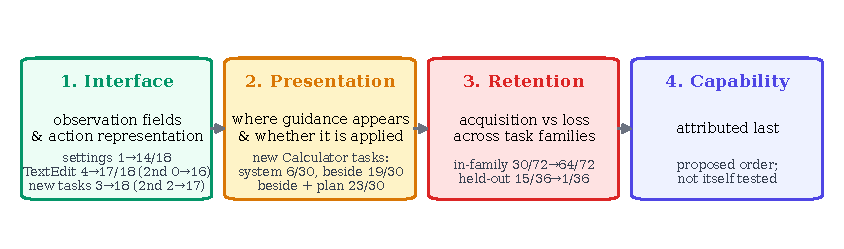
\includegraphics[width=0.92\linewidth,height=\textheight,keepaspectratio,alt={Working procedure used in this study. Each box lists the layer examined and its principal evidence; parenthesized values are from the second student. The order is a proposed procedure, not an experimentally compared one.}]{figures/fig1_diagnostic_order.pdf}
\caption{Working procedure used in this study. Each box lists the layer
examined and its principal evidence; parenthesized values are from the
second student. The order is a proposed procedure, not an experimentally
compared one.}\label{fig:order}
\end{figure}

\subsection{2. System and evidence
boundaries}\label{system-and-evidence-boundaries}

Figure 2 shows the components and the information each one receives. The
student acts only through the interface; the checker evaluates the
environment outside the student's prompt; the teacher sees failures and
produces guidance or guided rollouts; consolidation turns verified
rollouts into an adapter that is evaluated without guidance.

\begin{figure}
\centering
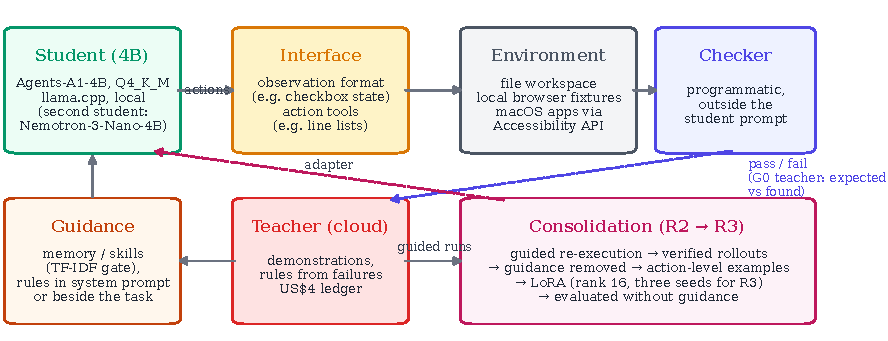
\includegraphics[width=0.92\linewidth,height=\textheight,keepaspectratio,alt={System overview. Solid arrows are the per-task loop; dashed arrows are training-time paths (checker verdicts to the teacher, and the trained adapter back to the student).}]{figures/fig0_system.pdf}
\caption{System overview. Solid arrows are the per-task loop; dashed
arrows are training-time paths (checker verdicts to the teacher, and the
trained adapter back to the student).}\label{fig:system}
\end{figure}

\textbf{Students.} The primary student is Agents-A1-4B in Q4\_K\_M
format (frozen revision \texttt{d92b02e2}, GGUF SHA-256
\texttt{d93c393a…f062}). File and browser evaluations ran on Kaggle T4
GPUs with a prebuilt llama.cpp (context 8,192 tokens for files, 16,384
for the browser); desktop evaluations ran on an Apple M4 Mac with
llama.cpp 0.4.1 (build 10964, context 8,192). The second student, used
only for the desktop replication in Sections 4--5, is NVIDIA
Nemotron-3-Nano-4B in Q4\_K\_M format (GGUF SHA-256
\texttt{be5d9a65…5ef2}) under the same server flags. Consolidation
training ran on a Colab A100.

\textbf{Execution budgets.} The file benchmark permits five loop steps,
six local model requests, twelve tool dispatches, and 150 s per attempt.
The browser protocol uses eight steps and ten model requests. Desktop
tasks have task-specific limits of six to twenty steps in the Desktop-v1
manifest, and the desktop loop issues one model request per step. These
are different protocols, not a common compute budget. File and desktop
runs use temperature 0.7; no result depends on temperature-zero
determinism.

\textbf{Learning and guidance.} After a failed file or browser attempt,
a teacher demonstration can be stored as trajectory memory or converted
into a parameterized skill verified in a sandbox. A TF-IDF gate selects
items by instruction similarity; when nothing passes, the request is
byte-identical to the raw student's. A separate mechanism asks the
teacher for one or two general rules, which are placed in the system
prompt or beside the task depending on the condition.

\textbf{Checker and teacher boundaries.} Programmatic checkers evaluate
outcomes outside the student's prompt. In the file and browser
experiments the teacher sees the checker's pass/fail verdict, not hidden
expected values. The desktop teacher is different: its prompts include
the training task's expected result and the observed checker finding, so
it receives privileged training feedback, not merely a binary reward;
the student receives the general rules, not test answers. The four
desktop rules were written from failures on four of the ten training
tasks (three TextEdit tasks and one Calculator chain task).
Student-unseen tasks may be developer-seen: inspecting evaluation
failures informed interface and prompt revisions, and the five desktop
variants were reused throughout development.

\textbf{Consolidation.} R2 collected guided rollouts on file and browser
tasks. Successful rollouts were converted to action-level supervised
examples after removing the guidance, split by task into training and
validation sets, and used for LoRA training (rank 16 on attention-output
and MLP projections, response-only loss, two epochs, learning rate
\(10^{-4}\), maximum sequence length 8,192, seed 0). Two further seeds
of R3 used the same data and hyperparameters (Section 6.2). Adapters
were evaluated without retrieved guidance or teacher assistance.

\textbf{Cost scope.} The cloud-teacher ledger is capped at US\$4.00 and
recorded US\$1.83 of cumulative use on 28 October 2026, including hosted
decision-model calls booked at list price (about US\$0.10) although they
ran within the provider's free allocation. Earlier project reports
quoted US\$1.12 (under an earlier US\$2.00 cap) and US\$1.78; these are
earlier snapshots of the same cumulative ledger, which is private and
was not audited by a second party. The five consolidation training
configurations total about 5.8 hours of wall time. GPU hours, student
inference, hardware, and developer effort are excluded.

\subsection{3. Benchmarks and analysis
protocol}\label{benchmarks-and-analysis-protocol}

Kage-Stream contains four learned file families (subset selection,
interval merge, log aggregation, CSV transformation), two families
excluded from consolidation training (text normalization and
configuration migration), and three read-only negative families. Its
evaluation set has 24 in-family, 12 held-out-family, and 12 negative
tasks. Kage-Web contains invoice, notification-settings, and
hotel-selection fixtures (18 learned tasks), a held-out profile-form
family, and read-only lookups; 30 tasks in all. Desktop-v1 contains
fifteen tasks: six Calculator, six TextEdit, and three read-only System
Settings tasks, split into ten training tasks and five variants.

\emph{Table 1. Evaluation units.}

{\def\LTcaptype{none} % do not increment counter
\begin{longtable}[]{@{}
  >{\raggedright\arraybackslash}p{(\linewidth - 4\tabcolsep) * \real{0.2000}}
  >{\raggedright\arraybackslash}p{(\linewidth - 4\tabcolsep) * \real{0.3176}}
  >{\raggedright\arraybackslash}p{(\linewidth - 4\tabcolsep) * \real{0.4824}}@{}}
\toprule\noalign{}
\begin{minipage}[b]{\linewidth}\raggedright
Experiment
\end{minipage} & \begin{minipage}[b]{\linewidth}\raggedright
Tasks
\end{minipage} & \begin{minipage}[b]{\linewidth}\raggedright
Repetition and interpretation
\end{minipage} \\
\midrule\noalign{}
\endhead
\bottomrule\noalign{}
\endlastfoot
E-1 (files) & 24 in-family, 12 held-out, 12 negative & two learning
streams; raw baseline evaluated once and reused \\
C4 (browser) & 30 (six per family) & three repeats per arm, same session
within a round \\
G0 (desktop) & 10 training + 5 variants & three repeats per task;
variants reused during development \\
G0 confirmation & 12 Calculator + 6 TextEdit, new & pre-registered;
three repeats; all arms interleaved in one session \\
R3 series & 24 learned-file, 12 held-out, 12 negative, 18 learned-web &
three repeats per adapter; three training seeds for R3, one for
R3b--R3e; single-run base anchors for R3b--R3e and the seed
replication \\
D7 (deployment) & 30 authored utterances per set & one prediction each;
intent label only \\
\end{longtable}
}

\textbf{Units.} An \emph{execution} is one attempt at one task; a
\emph{task} is one independent problem instance. Repeated executions are
not independent samples, and a repeated execution is not a new task.
Counts in tables are executions; tests are at the task level.
``In-family'' denotes new instances from the generators used for
practice (different seeds and parameters), so in-family gains are
same-generator generalization; the held-out families use different
generators.

\textbf{Task-level tests.} Repeats are averaged within a task, and
conditions are paired by task. We report the number of tasks that
improved, declined, or tied, and the exact two-sided sign-flip
probability of the mean within-task difference, computed by enumerating
all \(2^k\) sign assignments (by dynamic programming over integer-scaled
differences, so 24- and 30-task sets are exact as well). A 95\%
task-bootstrap interval (10,000 resamples) is descriptive only. The
minimum attainable value is \(2/2^{k'}\) for \(k'\) non-tied tasks: six
consistent tasks give \(1/32\), and three give \(1/4\). Values are
nominal: they are not corrected for the number of contrasts, they assume
exchangeable signs across tasks, and they condition on one trained
adapter. No execution-level Fisher tests are reported. Absence of a
detectable difference is not evidence of equivalence.

\textbf{Sessions and development status.} Within a C4 round and in the
original R3-versus-base comparison, arms ran in the same session.
R3b--R3e ran in later sessions, each with one base-model run as its
anchor. Task manifests were frozen before the main runs, but failures on
held-out families and on the desktop variants were inspected to design
later prompts, tools, and variants. All scores except those in Sections
4.2 and 5.4 marked as confirmation are development-set scores. For the
desktop suite we then collected a confirmation set: eighteen new tasks,
written and committed with the analysis plan, the frozen rules, and the
driver before any model ran on them (Section 5.4). No confirmation set
exists for the file and browser suites.

\subsection{4. Interface: observation and action
representation}\label{interface-observation-and-action-representation}

\subsubsection{4.1 Browser settings: one observation
field}\label{browser-settings-one-observation-field}

The compact browser observation omitted the \texttt{checked} key for
unchecked boxes. Settings tasks had resisted demonstrations, rules, and
consolidation, and we had described them as a case where the student
``knows but cannot do''. In C4 round 1, the raw student ran the frozen
web evaluation set under four interfaces with no learned guidance (Table
2).

\emph{Table 2. C4 browser interface ablation, round 1 (six settings
tasks; all 30 tasks; three repeats).}

{\def\LTcaptype{none} % do not increment counter
\begin{longtable}[]{@{}lrrl@{}}
\toprule\noalign{}
Interface & Settings (/18) & All tasks (/90) & Change from V1 \\
\midrule\noalign{}
\endhead
\bottomrule\noalign{}
\endlastfoot
V1: unchecked state implicit & 1 & 29 & --- \\
V2: explicit \texttt{checked:\ true/false} & 14 & 41 & one field \\
V2 + context packing & 14 & 36 & two changes \\
V2 + packing + state table & 17 & 39 & three changes \\
\end{longtable}
}

All six settings tasks improved from V1 to V2 (mean within-task
difference +0.72, bootstrap 0.50--0.94, \(p=1/32\), the smallest value
six tasks allow). Packing and the state table add no detectable
task-level difference over V2 (two improved, one declined, three tied;
\(p=1/2\)), so 17/18 is a composite, not a single-field estimate. In
round 2, the V2-plus-packing-plus-state-table configuration scored 18/18
on settings and 41/90 overall. A pre-save checker that compared
decision-model goal extractions with the page made no intervention in 59
checks; with settings at ceiling, this benchmark gives no evidence for
or against it.

Hotel failures persisted under every interface. Traces show the student
selecting a hotel without opening its rating details, with or without
context packing; we first blamed packing, and the corrected reading is
procedural. This is a trace-grounded hypothesis, not a demonstrated fix.

\subsubsection{4.2 Desktop TextEdit: action
representation}\label{desktop-textedit-action-representation}

With a whole-text \texttt{fill} action, TextEdit failures were mostly a
missing trailing newline or a literal \texttt{\textbackslash{}n} in the
JSON string, although the append and write instructions state the
newline requirement explicitly. Tools that let the program construct
line breaks removed these failures (Table 3).

\emph{Table 3. TextEdit tool interfaces on six tasks (three training,
three variants), three repeats each.}

{\def\LTcaptype{none} % do not increment counter
\begin{longtable}[]{@{}
  >{\raggedright\arraybackslash}p{(\linewidth - 10\tabcolsep) * \real{0.4262}}
  >{\raggedleft\arraybackslash}p{(\linewidth - 10\tabcolsep) * \real{0.1148}}
  >{\raggedleft\arraybackslash}p{(\linewidth - 10\tabcolsep) * \real{0.1148}}
  >{\raggedleft\arraybackslash}p{(\linewidth - 10\tabcolsep) * \real{0.1148}}
  >{\raggedleft\arraybackslash}p{(\linewidth - 10\tabcolsep) * \real{0.1148}}
  >{\raggedleft\arraybackslash}p{(\linewidth - 10\tabcolsep) * \real{0.1148}}@{}}
\toprule\noalign{}
\begin{minipage}[b]{\linewidth}\raggedright
Tool interface
\end{minipage} & \begin{minipage}[b]{\linewidth}\raggedleft
Fix (/6)
\end{minipage} & \begin{minipage}[b]{\linewidth}\raggedleft
Append (/6)
\end{minipage} & \begin{minipage}[b]{\linewidth}\raggedleft
Write (/6)
\end{minipage} & \begin{minipage}[b]{\linewidth}\raggedleft
Primary (/18)
\end{minipage} & \begin{minipage}[b]{\linewidth}\raggedleft
Second student (/18)
\end{minipage} \\
\midrule\noalign{}
\endhead
\bottomrule\noalign{}
\endlastfoot
Whole-text \texttt{fill} & 0 & 3 & 1 & 4 & 0 \\
+ \texttt{replace\_text}, \texttt{append\_text} (v3) & 6 & 2 & 0 & 8 &
--- \\
Line-list actions (v4), no lessons & 6 & 5 & 6 & 17 & 16 \\
v4 + four lessons + plan (final) & 5 & 4 & 6 & 15 & 14/17\(^a\) \\
\end{longtable}
}

\(^a\) One setup error (document window missing) excluded. The primary
student's \texttt{fill} row combines training runs under interface v1
with variant runs under v2; both of the second student's \texttt{fill}
runs are under v2.

For both students all six tasks improve from \texttt{fill} to v4
(primary: mean +0.72, \(p=1/32\); second student: mean +0.89,
\(p=1/32\)). For the primary student, v4 improves four tasks over v3 and
ties two (\(p=1/8\)). Adding the lessons and the plan at the same
interface leaves four tasks unchanged and lowers two by one execution
each (0/2/4, \(p=1/2\)); the second student shows the same pattern
(0/1/5, \(p=1\)). The data therefore show no observed TextEdit increment
from the lesson component once the interface is fixed, which is not the
same as showing that the lessons are useless or harmful.

On six new TextEdit tasks of the pre-registered confirmation (Section
5.4), with no lessons and both interfaces interleaved in one session,
\texttt{fill} scored 3/18 and v4 18/18 for the primary student, and 2/18
and 17/18 for the second student; all six tasks improved for each
student (mean +0.83, \(p=1/32\), the minimum attainable with six tasks).
The failures under \texttt{fill} were again missing trailing newlines.

\begin{figure}
\centering
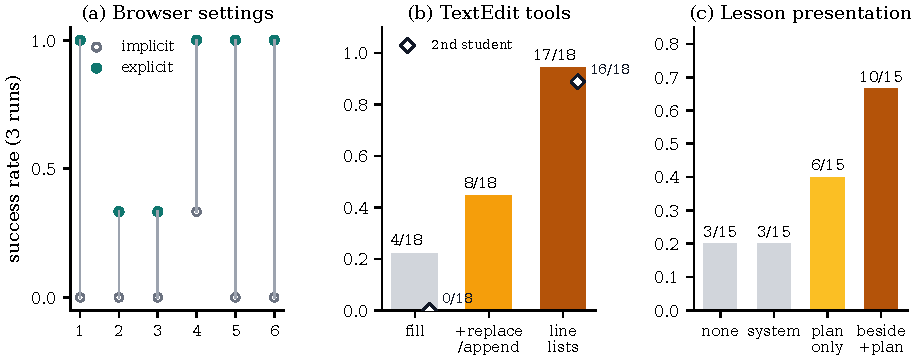
\includegraphics[width=0.92\linewidth,height=\textheight,keepaspectratio,alt={Interventions at three layers. (a) Browser settings per task under implicit (open) and explicit (filled) checkbox state, three repeats per task. (b) TextEdit tool interfaces; bars are the primary student, diamonds the second student; the primary fill bar mixes interface v1 training runs and v2 variant runs. (c) Desktop lesson-presentation pilot for the primary student on five variants, three repeats each; the second student scored 0--1/15 in every condition (Table 5).}]{figures/fig2_interventions.pdf}
\caption{Interventions at three layers. (a) Browser settings per task
under implicit (open) and explicit (filled) checkbox state, three
repeats per task. (b) TextEdit tool interfaces; bars are the primary
student, diamonds the second student; the primary \protect\texttt{fill}
bar mixes interface v1 training runs and v2 variant runs. (c) Desktop
lesson-presentation pilot for the primary student on five variants,
three repeats each; the second student scored 0--1/15 in every condition
(Table 5).}\label{fig:interventions}
\end{figure}

\subsubsection{4.3 The final desktop
configuration}\label{the-final-desktop-configuration}

Line-oriented tools, reference-handling fixes, and task-adjacent lessons
with planning together scored 41/45 executions for the primary student:
29/30 on the training tasks and 12/15 on the variants (Calculator 17/18,
TextEdit 15/18, read-only System Settings 9/9). The earlier baselines
were 19/30 on the training tasks under interface v1 without rules and
3/15 on the variants under interface v2 without rules. This is a
configuration result. Table 4 lists the observed change on the training
tasks by family together with the control that exists for it; it is not
an attribution of the ten-point gain.

\emph{Table 4. Final configuration versus baseline on the ten training
tasks (three repeats), by family.}

{\def\LTcaptype{none} % do not increment counter
\begin{longtable}[]{@{}
  >{\raggedright\arraybackslash}p{(\linewidth - 8\tabcolsep) * \real{0.1889}}
  >{\raggedleft\arraybackslash}p{(\linewidth - 8\tabcolsep) * \real{0.0778}}
  >{\raggedleft\arraybackslash}p{(\linewidth - 8\tabcolsep) * \real{0.0778}}
  >{\raggedright\arraybackslash}p{(\linewidth - 8\tabcolsep) * \real{0.3222}}
  >{\raggedright\arraybackslash}p{(\linewidth - 8\tabcolsep) * \real{0.3333}}@{}}
\toprule\noalign{}
\begin{minipage}[b]{\linewidth}\raggedright
Family
\end{minipage} & \begin{minipage}[b]{\linewidth}\raggedleft
Baseline v1, no rules
\end{minipage} & \begin{minipage}[b]{\linewidth}\raggedleft
Final
\end{minipage} & \begin{minipage}[b]{\linewidth}\raggedright
Matched control
\end{minipage} & \begin{minipage}[b]{\linewidth}\raggedright
Compatible explanation
\end{minipage} \\
\midrule\noalign{}
\endhead
\bottomrule\noalign{}
\endlastfoot
TextEdit (3) & 2/9 & 8/9 & v4 without lessons: 8/9 & line-oriented
tools; no observed lesson increment \\
Settings (3) & 7/9 & 9/9 & none & the two baseline failures were a
missing tool call and a whole-line reference, the cases the v2 fixes
handle; no settings lessons existed, but the plan instruction applies \\
Calculator (4) & 10/12 & 12/12 & none & the gain is on the chain task
whose failure produced the Calculator lesson (in-sample); lesson and
plan not separated \\
\textbf{Total} & \textbf{19/30} & \textbf{29/30} & & composite \\
\end{longtable}
}

Only the TextEdit change has a matched control. The settings change is
consistent with the interface fixes by trace evidence but was not
measured in isolation, and the Calculator change is an in-sample
improvement that could come from the lesson, the plan, or run variation.
A full fifteen-task v4 arm without lessons, interleaved with the final
configuration in one session, is the most informative missing control.

The second student reached 18/44 executions under the same final
configuration (Calculator 0/18, TextEdit 14/17, System Settings 4/9).
Its Calculator failures were not repaired by any interface or prompt
tested. Under the default references it pressed digit keys that did not
match the operands (for 1234 + 5678 it began with 7, 8, 4); when
references were replaced by control identifiers (interface v5) it
pressed the digit keys in their listed order (Seven, Eight, Nine, Four,
\ldots). Calculator scored 0/18 under v5 as well. We first read the
default-reference behavior as confusing reference numbers with digits;
the v5 result does not support that reading.

\subsection{5. Presentation-dependent
adoption}\label{presentation-dependent-adoption}

\subsubsection{5.1 Demonstrations help within a
family}\label{demonstrations-help-within-a-family}

In E-1, after a 60-task learning stream, trajectory memory achieved
42/48 in-family executions and a skill library 39/48, compared with
14/48 for the raw baseline and 12/48 for budget-matched retries; the
learning arms combine two streams evaluated on the same 24 tasks, and
the raw baseline is one evaluation duplicated for the comparison. At the
task level, memory improved 17 tasks and lowered one (mean +0.58,
bootstrap 0.35--0.79, \(p=25/131{,}072\)), and the skill library
improved 14 and lowered none (+0.52, \(p=1/8{,}192\)); memory and skills
do not differ detectably (5/4/15, \(p=43/64\)). On the twelve held-out
tasks memory did not improve over the raw student (2/4/6, \(p=1/2\)).
Later single raw evaluations of the same 24 tasks ranged from 6 to 13
successes, which bounds how much of the difference a lucky baseline
could explain but does not replace repeated baselines. Demonstrations
taught same-generator procedures, not cross-family transfer.

\subsubsection{5.2 Retrieval without
enactment}\label{retrieval-without-enactment}

On browser tasks, retrieved guidance was not consistently enacted. In C2
the relevant demonstration was present in the evaluation prompt, yet the
student solved only a minority of invoice tasks, concentrated on the
same two tasks. In C3, teacher-written procedural rules were injected
through the system prompt (TF-IDF gated, at most two rules), and invoice
tasks rose from 0/24 to 14/24 executions: a missing-step failure
repaired by a rule. The same delivery did not help settings tasks, whose
failure was later traced to the observation field of Section 4.1, and
hotel tasks remained procedural.

This appears to conflict with the desktop pilot below, where
system-prompt rules did nothing. The two differ in more than delivery:
the C3 rules supplied a missing step and were relevance-gated, whereas
the desktop rules concerned action representation (line breaks) and
Calculator operator order. We do not isolate content type, retrieval,
number of rules, or planning.

\subsubsection{5.3 The desktop lesson
pilot}\label{the-desktop-lesson-pilot}

Calculator chain tasks exposed a missing procedure: entering an addition
followed by a multiplication without first resolving the addition gives
the wrong grouping. The teacher wrote one rule about pressing Equals
after the addition and three about preserving text and newlines. On the
five variants, which were not used to write the rules, four conditions
were compared under interface v2 (Table 5).

\emph{Table 5. Desktop lesson pilot: five variants, three repeats each
(executions).}

{\def\LTcaptype{none} % do not increment counter
\begin{longtable}[]{@{}
  >{\raggedright\arraybackslash}p{(\linewidth - 8\tabcolsep) * \real{0.2000}}
  >{\raggedleft\arraybackslash}p{(\linewidth - 8\tabcolsep) * \real{0.2000}}
  >{\raggedleft\arraybackslash}p{(\linewidth - 8\tabcolsep) * \real{0.2000}}
  >{\raggedleft\arraybackslash}p{(\linewidth - 8\tabcolsep) * \real{0.2000}}
  >{\raggedleft\arraybackslash}p{(\linewidth - 8\tabcolsep) * \real{0.2000}}@{}}
\toprule\noalign{}
\begin{minipage}[b]{\linewidth}\raggedright
Prompt condition
\end{minipage} & \begin{minipage}[b]{\linewidth}\raggedleft
Primary: Calc. (/6)
\end{minipage} & \begin{minipage}[b]{\linewidth}\raggedleft
Primary: TextEdit (/9)
\end{minipage} & \begin{minipage}[b]{\linewidth}\raggedleft
Primary total (/15)
\end{minipage} & \begin{minipage}[b]{\linewidth}\raggedleft
Second student (/15)
\end{minipage} \\
\midrule\noalign{}
\endhead
\bottomrule\noalign{}
\endlastfoot
No lessons & 1 & 2 & 3 & 0 \\
Lessons in system prompt & 1 & 2 & 3 & 1 \\
Plan first, no lessons & 4 & 2 & 6 & 0 \\
Lessons beside task; explain application, then act & 5 & 5 & 10 & 0 \\
\end{longtable}
}

For the primary student the combined condition is numerically strongest,
and planning alone accounts for much of the Calculator change. Against
no lessons, the combined condition improves three tasks and ties two
(mean +0.47, bootstrap 0.13--0.80, \(p=1/4\)); plan only improves two
and ties three (\(p=1/2\)); lessons in the system prompt are exactly
neutral on average (\(p=1\)); and the combined condition improves two
tasks over plan only and ties three (\(p=1/2\)). The combined condition
changes lesson placement and adds an application step, so it does not
isolate rule content, location, or deliberation. The second student's
lessons were written from its own failures and were generic (``clear the
display, verify the expression''), and every condition scored 0 or 1 of
15. The pilot therefore shows that the same rules can be ignored in one
presentation and used in another by the primary student; it does not
establish a general effect.

\subsubsection{5.4 Pre-registered
confirmation}\label{pre-registered-confirmation}

The pilot confounded placement with planning and reused variants that
the developer had inspected. We therefore wrote twelve new Calculator
tasks and six new TextEdit tasks, verified them with scripted solutions
(18/18), and committed the tasks, the four frozen rules from Section
5.3, the driver, and an analysis plan with four primary contrasts before
the first model run. Ten Calculator tasks require grouping, as in
\((61-25)\times 3\); two \emph{precedence controls} (\(8+7\times 6\),
\(12+9\times 3\)) are solved by typing straight through, so pressing
Equals after the addition, as the rule advises, gives the wrong answer.
Five conditions ran under interface v4: no rule, rule in the system
prompt, plan only, rule beside the task without a plan request (new),
and rule beside the task with the application plan. For every task and
repeat, all conditions ran back to back in a rotated order, so time and
application state are spread across conditions. Two executions failed in
setup three times (Calculator had no window) and count as failures, as
pre-registered; excluding them changes only the second contrast, to
7/0/3 and \(p=1/64\).

\emph{Table 6. Pre-registered desktop confirmation, primary student,
three repeats per task (executions).}

{\def\LTcaptype{none} % do not increment counter
\begin{longtable}[]{@{}lrr@{}}
\toprule\noalign{}
Condition & Grouping (/30) & Precedence controls (/6) \\
\midrule\noalign{}
\endhead
\bottomrule\noalign{}
\endlastfoot
No rule & 1 & 6 \\
Rule in system prompt & 6 & 6 \\
Plan only & 12 & 6 \\
Rule beside task, no plan & 19 & 4 \\
Rule beside task, plan & 23 & 4 \\
\end{longtable}
}

The four pre-registered contrasts on the ten grouping tasks
(improved/declined/tied, exact \(p\)) are: beside with plan versus no
rule, 10/0/0, \(p=1/512\); beside without plan versus system prompt,
8/0/2, \(p=1/128\); beside with plan versus plan only, 6/1/3,
\(p=1/16\); and beside with plan versus beside without plan, 5/1/4,
\(p=7/32\). The first two meet the pre-registered criterion (\(p<0.05\)
in the predicted direction); the last two do not. The combined condition
of the pilot therefore replicates on new tasks, but most of its effect
comes from where the rule appears: placing it beside the task, without
asking for a plan, raised success from 6/30 to 19/30, while the plan's
further increment was not detectable. On the precedence controls, the
three conditions without a task-adjacent rule scored 18/18 and the two
with one scored 8/12; three of the four failures pressed Equals after
the addition, producing \((12+9)\times 3\) or \((8+7)\times 6\). The
second student was not run on these Calculator tasks, because it had
scored 0 in every earlier Calculator condition (0/108 executions), and
the plan said so before the run.

These results narrow C2: for this student and this rule, placement
beside the task governs adoption, and it governs it indiscriminately.
They do not separate position in the context from framing as part of the
request, and they rest on one rule, one family, one student, and one
session.

\begin{figure}
\centering
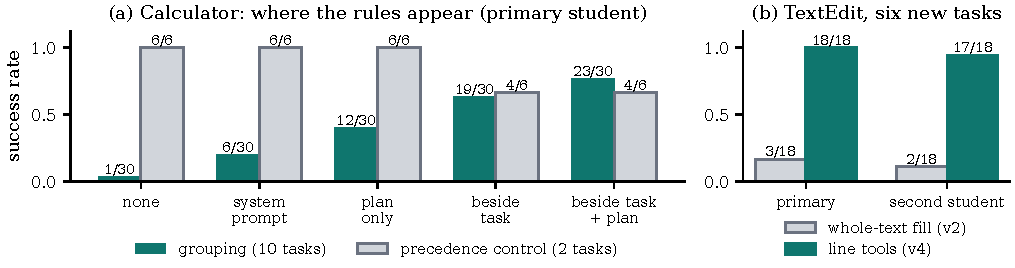
\includegraphics[width=0.92\linewidth,height=\textheight,keepaspectratio,alt={Pre-registered confirmation on new tasks. (a) Calculator, primary student: ten grouping tasks and two precedence controls, three repeats each, under five presentations of the same rule. (b) TextEdit, six tasks, three repeats, for both students.}]{figures/fig4_confirmation.pdf}
\caption{Pre-registered confirmation on new tasks. (a) Calculator,
primary student: ten grouping tasks and two precedence controls, three
repeats each, under five presentations of the same rule. (b) TextEdit,
six tasks, three repeats, for both students.}\label{fig:confirm}
\end{figure}

\subsection{6. Consolidation and
retention}\label{consolidation-and-retention}

\subsubsection{6.1 Data and training
units}\label{data-and-training-units}

The R2 archive contains 1,900 action-level examples from 151 unique task
IDs. Each row pairs a conversation context with a target response, and
one successful rollout can contribute several rows. The four collection
reports record 704 attempts and 472 successes before filtering, and the
retained archive contains 446 distinct task/source/attempt combinations;
none of these counts is a number of independent tasks. R3 splits the
archive by task into 1,677 training and 223 validation examples. Replay
data come from AgentNet desktop-action steps (Wang et al., 2025; 800
examples) and Toucan MCP tool calls (Xu et al., 2025; 600 examples);
neither contains code-writing steps. Table 7 lists the training exposure
of each variant.

\emph{Table 7. Training exposure (saved training configurations; seed 0,
two epochs).}

{\def\LTcaptype{none} % do not increment counter
\begin{longtable}[]{@{}
  >{\raggedright\arraybackslash}p{(\linewidth - 8\tabcolsep) * \real{0.2000}}
  >{\raggedright\arraybackslash}p{(\linewidth - 8\tabcolsep) * \real{0.2000}}
  >{\raggedleft\arraybackslash}p{(\linewidth - 8\tabcolsep) * \real{0.2000}}
  >{\raggedleft\arraybackslash}p{(\linewidth - 8\tabcolsep) * \real{0.2000}}
  >{\raggedleft\arraybackslash}p{(\linewidth - 8\tabcolsep) * \real{0.2000}}@{}}
\toprule\noalign{}
\begin{minipage}[b]{\linewidth}\raggedright
Version
\end{minipage} & \begin{minipage}[b]{\linewidth}\raggedright
Main change
\end{minipage} & \begin{minipage}[b]{\linewidth}\raggedleft
Training examples
\end{minipage} & \begin{minipage}[b]{\linewidth}\raggedleft
Replay
\end{minipage} & \begin{minipage}[b]{\linewidth}\raggedleft
Optimizer steps
\end{minipage} \\
\midrule\noalign{}
\endhead
\bottomrule\noalign{}
\endlastfoot
R3 & guided-success targets & 1,677 & 0 & 420 \\
R3b & filter reasoning-free targets; random replay & 2,781 & 1,400 &
696 \\
R3c & filter; LESS-selected replay & 2,266 & 879 & 567 \\
R3d & restore targets with teacher rationales; LESS replay & 2,736 & 879
& 684 \\
R3e & rationales; random replay & 3,251 & 1,400 & 813 \\
\end{longtable}
}

R3e's configuration lists 3,257 rows, six of which exceed the
8,192-token limit, leaving 3,251 trained examples.

\subsubsection{6.2 Acquisition and loss}\label{acquisition-and-loss}

\emph{Table 8. Consolidation results (executions; three inference runs
per adapter). Anchors are untrained base runs from the same session:
three runs for R3, one run for R3b--R3e.}

{\def\LTcaptype{none} % do not increment counter
\begin{longtable}[]{@{}
  >{\raggedright\arraybackslash}p{(\linewidth - 10\tabcolsep) * \real{0.1296}}
  >{\raggedright\arraybackslash}p{(\linewidth - 10\tabcolsep) * \real{0.3519}}
  >{\raggedleft\arraybackslash}p{(\linewidth - 10\tabcolsep) * \real{0.1296}}
  >{\raggedleft\arraybackslash}p{(\linewidth - 10\tabcolsep) * \real{0.1296}}
  >{\raggedleft\arraybackslash}p{(\linewidth - 10\tabcolsep) * \real{0.1296}}
  >{\raggedleft\arraybackslash}p{(\linewidth - 10\tabcolsep) * \real{0.1296}}@{}}
\toprule\noalign{}
\begin{minipage}[b]{\linewidth}\raggedright
Version
\end{minipage} & \begin{minipage}[b]{\linewidth}\raggedright
Anchor in / held-out
\end{minipage} & \begin{minipage}[b]{\linewidth}\raggedleft
Learned files (/72)
\end{minipage} & \begin{minipage}[b]{\linewidth}\raggedleft
Held-out files (/36)
\end{minipage} & \begin{minipage}[b]{\linewidth}\raggedleft
Learned web (/54)
\end{minipage} & \begin{minipage}[b]{\linewidth}\raggedleft
Negative skill misuse (/36)
\end{minipage} \\
\midrule\noalign{}
\endhead
\bottomrule\noalign{}
\endlastfoot
Base (R3 anchor) & 30/72 · 15/36 & 30 & 15 & 10 & 0 \\
R3 & same as base & 64 & 1 & 21 & 2 \\
R3b & 10/24 · 7/12 & 34 & 15 & 31 & 0 \\
R3c & 11/24 · 7/12 & 34 & 2 & 22 & 0 \\
R3d & 6/24 · 5/12 & 62 & 6 & 20 & 0 \\
R3e & 11/24 · 7/12 & 65 & 1 & 22 & 0 \\
\end{longtable}
}

In the same-session R3 comparison, the in-family gain appears in every
repeat (22, 22, 20 of 24 versus 9, 12, 9) and so does the held-out
decline (1, 0, 0 of 12 versus 5, 5, 5). At the task level, 14 in-family
tasks improved, 2 declined, and 8 tied (mean +0.47, bootstrap
0.28--0.67, \(p=11/32{,}768\)); among held-out tasks 6 declined, 1
improved, and 5 tied (−0.39, bootstrap −0.67 to −0.11, \(p=3/64\)).
Learned web tasks improved on 7 and declined on 2 (+0.20, \(p=7/64\)).
Against their single-run anchors, R3d and R3e show the same pattern
(in-family \(p=1/32{,}768\) and \(3/4{,}096\); held-out −0.25,
\(p=33/128\), and −0.56, \(p=1/64\)), whereas R3b and R3c show no
detectable in-family gain (+0.06 and +0.01) with held-out differences of
−0.17 (\(p=131/256\)) and −0.53 (\(p=1/64\)). Single-run anchors are
noisier than the three-run base, so these variant contrasts are
descriptive.

\textbf{Training seeds.} To test whether the R3 result depends on one
training run, we retrained R3 with seeds 1 and 2 on the same 1,677
examples (identical data hash) and hyperparameters. Only the hardware
differed: seed 0 was trained on an A100 in bf16, seeds 1 and 2 on a T4
in fp16, with exactly computed causal attention in query blocks of 1,024
tokens to fit the 8,192-token limit in 16 GB. Both adapters were
evaluated in one later session under the R3 protocol, with one base run
as the anchor (Table 9).

\emph{Table 9. R3 training seeds (executions; three inference runs per
adapter).}

{\def\LTcaptype{none} % do not increment counter
\begin{longtable}[]{@{}
  >{\raggedright\arraybackslash}p{(\linewidth - 12\tabcolsep) * \real{0.1429}}
  >{\raggedright\arraybackslash}p{(\linewidth - 12\tabcolsep) * \real{0.1429}}
  >{\raggedleft\arraybackslash}p{(\linewidth - 12\tabcolsep) * \real{0.1429}}
  >{\raggedleft\arraybackslash}p{(\linewidth - 12\tabcolsep) * \real{0.1429}}
  >{\raggedleft\arraybackslash}p{(\linewidth - 12\tabcolsep) * \real{0.1429}}
  >{\raggedleft\arraybackslash}p{(\linewidth - 12\tabcolsep) * \real{0.1429}}
  >{\raggedleft\arraybackslash}p{(\linewidth - 12\tabcolsep) * \real{0.1429}}@{}}
\toprule\noalign{}
\begin{minipage}[b]{\linewidth}\raggedright
Adapter
\end{minipage} & \begin{minipage}[b]{\linewidth}\raggedright
Training
\end{minipage} & \begin{minipage}[b]{\linewidth}\raggedleft
Learned files (/72)
\end{minipage} & \begin{minipage}[b]{\linewidth}\raggedleft
Held-out files (/36)
\end{minipage} & \begin{minipage}[b]{\linewidth}\raggedleft
Learned web (/54)
\end{minipage} & \begin{minipage}[b]{\linewidth}\raggedleft
Negative skill misuse (/36)
\end{minipage} & \begin{minipage}[b]{\linewidth}\raggedleft
General (/30)
\end{minipage} \\
\midrule\noalign{}
\endhead
\bottomrule\noalign{}
\endlastfoot
R3, seed 0 & A100, bf16 & 64 (22, 22, 20) & 1 (1, 0, 0) & 21 & 2 & 28 \\
R3, seed 1 & T4, fp16 & 63 (21, 21, 21) & 0 (0, 0, 0) & 26 & 0 & 28 \\
R3, seed 2 & T4, fp16 & 58 (20, 19, 19) & 2 (1, 1, 0) & 28 & 1 & 28 \\
Base, seed-session anchor (1 run) & --- & 10/24 & 5/12 & 3/18 & 0/12 &
--- \\
\end{longtable}
}

Both seeds reproduce both effects. Against the same-session anchor, seed
1 gained in-family (+0.46; 13 tasks improved, 2 declined;
\(p=121/16{,}384\)) and lost on held-out families (−0.42; 0 improved, 5
declined; \(p=1/16\)); seed 2 likewise (+0.39, 12/3, \(p=79/8{,}192\);
−0.36, 2/5, \(p=1/16\)). With five or seven untied held-out tasks
against a single anchor run, \(p=1/16\) is close to the smallest
attainable value. The anchor matched the earlier three-run base exactly
in totals (10/24 and 5/12 against 30/72 and 15/36), and against that
base the held-out decline is \(p=1/32\) for seed 1 and \(1/16\) for seed
2; averaging the two seeds, 15 in-family tasks improved and 1 declined
(\(p=27/32{,}768\)), and 6 held-out tasks declined and 2 improved
(\(p=5/128\)). Neither seed differs detectably from seed 0 (in-family
−0.01 and −0.08, \(p=1\) and \(59/128\); held-out −0.03 and +0.03,
\(p=1\)). Learned web tasks also improved for both (+0.32 and +0.35;
\(p=9/256\) and \(11/512\)). Seed 2 made one skill call on the same
read-only look-alike family that seed 0 misused. The trade-off is
therefore not an artifact of one training run; it remains a result for
one dataset, one model, and one hyperparameter setting.

R3 also issued skill calls on read-only negative tasks in 2 of 36
executions; both were on the same look-alike task (two of its three
runs) and failed it, and neither run wrote a file. The base model and
R3b--R3e issued none. Under the round-2 browser interface, R3e achieved
7/18 invoice executions versus 0/18 for the same-interface raw arm and
47/90 versus 41/90 overall; at the task level the overall gain comes
from three tasks, all invoices (three improved, one declined, 26 tied;
\(p=1/4\)). Some invoice behavior survives the interface change; broad
interface-invariant transfer is not shown. A 30-question general-ability
check scored 27--28 across variants, too small to establish preservation
of general capability.

\begin{figure}
\centering
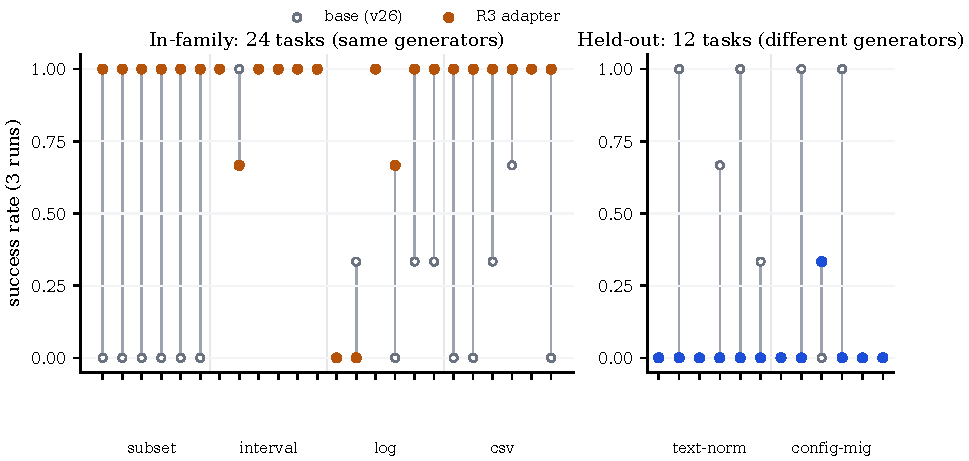
\includegraphics[width=0.92\linewidth,height=\textheight,keepaspectratio,alt={Per-task success of the base model (open) and the R3 adapter (filled), three runs each. Left: 24 in-family tasks, of which 14 improved, 2 declined, and 8 tied. Right: 12 held-out-family tasks, of which 6 declined, 1 improved, and 5 tied.}]{figures/fig3_r3_per_task.pdf}
\caption{Per-task success of the base model (open) and the R3 adapter
(filled), three runs each. Left: 24 in-family tasks, of which 14
improved, 2 declined, and 8 tied. Right: 12 held-out-family tasks, of
which 6 declined, 1 improved, and 5 tied.}\label{fig:r3}
\end{figure}

\subsubsection{6.3 What the variants do not
identify}\label{what-the-variants-do-not-identify}

Filtering reasoning-free targets disproportionately removed file
solutions: the learned families contain 202 reasoning-free
\texttt{write\_file} targets and 101 with reasoning (102 including one
negative-family row), so the filter did not remove every file-writing
example. Restoring the filtered targets with teacher-written rationales
recovered most of the in-family gain while held-out success stayed low
(R3d, R3e). This rules out the account that restoring visible reasoning
text is sufficient to prevent the degradation in these configurations.

It does not show that gain and loss share a single cause. R3b and R3c
filter the same targets and reach the same 34/72 in-family, yet their
held-out results differ (15/36 versus 2/36). They also differ in replay
algorithm, replay size (1,400 versus 879), source mixture, and optimizer
steps (696 versus 567), so the contrast shows that retention is not a
function of filtering alone, not that replay selection is responsible.
R3b's held-out 15/36 equals the three-run base from the R3 session and
lies below its own single-run anchor (7/12, i.e.~21/36 at that rate);
the difference is not detectable at the task level (\(p=131/256\)), and
R3b also kept little of the in-family gain.

Trace analyses report less reading back of written files and plausible
but incorrect code after training. Reduced verification is a candidate
mechanism, not an established cause: no intervention forced read-back
while holding model and task fixed, and R3b retained more held-out
success despite reduced verification. Testing it requires controlled
verification interventions and training data that keep successful
checking steps; testing replay explanations requires matched amounts,
source composition, exposure, and several training seeds per variant
(only R3 has more than one). None of these experiments is claimed here.

\subsection{7. Second student}\label{second-student}

The desktop replication with Nemotron-3-Nano-4B ran the G0 protocol
unattended in one session, with lessons written by the same teacher from
the second student's own training failures (US\$0.0014). Two earlier
attempts were void and are excluded: one failed in Calculator setup when
the display was not clear, and one ran after the screen locked, which
disables Accessibility actions. Its training-task baseline was 3/30
under interface v2 (primary student: 19/30 under v1). Three observations
follow. The TextEdit tool effect reproduced (Table 3) and held on the
new confirmation tasks (2/18 to 17/18). The presentation effect did not
(Table 5). The Calculator failure was specific to this student and
survived two interface changes (Section 4.3). The replication covers one
model and one session and was not reviewed by a second person; it
narrows C1 to a tool-representation effect seen in two students and C2
to the primary student.

\subsection{8. Discussion}\label{discussion}

\textbf{Why interfaces matter more for small students.} The two
interface failures share a structure: the information the student needed
was present but had to be inferred or encoded. In the V1 browser
observation an unchecked box was signalled by the \emph{absence} of a
key, while the same entry still carried \texttt{"value":\ "on"}
(Appendix B.1); a larger model may infer the convention, but a 4B
student reads what is written. In whole-text editing, a line break had
to be emitted as an escape sequence inside a JSON string, and the
student produced either nothing or a literal backslash-n even when its
own plan stated the requirement. In both cases the repair removed an
inference or an encoding step instead of teaching one. This suggests a
cheap diagnostic before collecting data or training: hold the guidance
fixed and change only the representation of the observation or action.
In our runs, a failure that moved under such a change was not a
capability gap, and the repair was a one-time engineering change rather
than a recurring data cost.

\textbf{Placement decides whether a rule is used, and where.} For the
primary student, the same rule was mostly ignored in the system prompt
and used when it sat beside the task; asking for an application plan
added little once the rule was there. The same placement made the
student apply the rule to expressions where it did not hold. A rule
beside the task thus acts less like advice the student weighs and more
like an instruction it follows, so deployed rules need stated conditions
of use and should be tested on cases where they do not apply.
\textbf{Guidance needs a competence floor.} The second student did not
benefit from any presentation: it could not map an arithmetic expression
onto Calculator keys, and no rule about operator order could repair
that. Presentation effects are therefore conditional on the student
already being able to carry out the underlying actions; where that floor
is missing, the failure belongs to an earlier layer (here, grounding
operands to controls) that rules do not reach.

\textbf{Measuring retention is cheap; skipping it is not.} The in-family
gains came from new instances of the same generators, which is a narrow
form of generalization, and the two excluded families exposed losses
that in-family scores alone would have hidden. Evaluating excluded
families and read-only negatives after every weight change cost little
relative to training. In deployment we therefore kept learning in
context (memory, skills, and rules behind a relevance gate) rather than
shipping a consolidated adapter; family-gated adapters are an untested
alternative.

\textbf{Privileged teacher feedback can reach the student.} The desktop
teacher saw expected values and checker findings, and one of the rules
it wrote for the student cites the checker directly (``since the checker
requires each line to be newline-terminated'', Appendix B.3). The rule
is general and contains no test answer, but it shows that feedback given
to a teacher can shape what the student is told. Evaluations that
separate student-visible from teacher-visible information should inspect
the generated guidance, not only the prompts.

\subsection{9. Related work}\label{related-work}

\textbf{Computer-use benchmarks.} OSWorld evaluates multimodal agents on
open-ended tasks in real desktop environments (Xie et al., 2024), and
WebArena on self-hosted websites (Zhou et al., 2024); both report large
gaps between the strongest agents and humans. Our suites are smaller and
procedurally generated so that families can be held out of training and
failures inspected one interface field at a time; they are not a
substitute for these benchmarks.

\textbf{Interfaces.} SWE-agent studies agent-computer interface design
and shows that tools adapted to language-model agents improve
software-engineering performance (Yang et al., 2024). Our narrower
contribution is a diagnostic study in which explicit checkbox state and
line-oriented actions address observed small-model failure modes; we do
not claim interface design as a new principle. GUI toggle state has
independently been identified as a failure point for multimodal agents
(Wu et al., 2026). The ARTEMIS Android automation project prompted our
interface ablation.

\textbf{Experience and consolidation.} Agent Workflow Memory induces and
retrieves reusable procedures (Wang et al., 2025). Context distillation
transfers information supplied in context into model behavior (Snell et
al., 2022). Kage's guided re-execution draws on the recursive
self-rewrite component of Terminal-RSI (Yang et al., 2026), but not its
reinforcement-learning stages or a second training round. Our rationale
step is related to STaR (Zelikman et al., 2022), except that a teacher
writes rationales for existing targets. Harness search changes the
scaffolding around a model rather than its weights (Meta-Harness, Lee et
al., 2026; Harness\(^2\), Xu et al., 2026); the interface changes
reported here were made by the developer.

\textbf{Retention and data selection.} Biderman et al.~(2024) compare
LoRA with full fine-tuning and find that LoRA learns less and forgets
less; this is a relative comparison, it does not imply that LoRA avoids
forgetting, and we have no full-fine-tuning comparator. LESS selects
examples aligned with a target capability (Xia et al., 2024); our
unequal-size replay comparison cannot establish a general limitation of
LESS as an anti-forgetting method. Forgetting from synthetic fine-tuning
data has been reported for the retrieval component of LLM-agent skill
systems (Murtaza et al., 2026), and cross-environment transfer of
fine-tuned agents has been studied in relation to observation and action
shifts (Xi et al., 2026).

\textbf{Position of information in context.} Language models use
information less reliably when it sits in the middle of long contexts
than at the beginning or end (Liu et al., 2024). Moving rules from the
system prompt to beside the task changes their position as well as their
framing; our confirmation separates placement from planning but not
position from framing.

\textbf{Statistical practice.} Our task-level analysis follows the
argument that significance tests must respect the unit of independent
sampling (Dror et al., 2018).

\subsection{10. Limitations and reproduction
status}\label{limitations-and-reproduction-status}

The study uses one primary model, a partial desktop replication with a
second, three training seeds for the main adapter but one for each
variant, procedural task families, a small desktop suite, and one user's
deployment. Repeated runs characterize inference variability but do not
add independent tasks; the two extra R3 seeds were trained in fp16 on
different hardware from seed 0, so seed and precision are not separated.
Developer inspection of evaluation failures influenced later prompts,
tools, and training variants. A pre-registered confirmation exists only
for the desktop tool and rule-placement results; it covers one rule
family, eighteen developer-written tasks, and one session per student.
Cross-session single-run anchors for R3b--R3e, unequal training exposure
across variants, a composite final desktop configuration, and nominal
tests without multiplicity correction further limit causal
interpretation.

\textbf{Deployment note.} In daily use, a hosted decision model (Clef)
routed requests to program handlers and matched the intent label on
30/30 utterances in each of two authored sets, against 15/30 and 16/30
for the pattern router it replaced; with a 0.8 confidence fallback to
the local model, 30/30 and 28/30. These are intent-label matches only,
not completed tasks: one second-set date label is itself wrong, the
first set was reused as development data for the second router, there is
no matched 4B router baseline, and request text leaves the machine for
routing. Before-and-after cases from the private activity log (a weather
question from 36.5 s to 0.8 s; a knowledge question from a failed 16 s
tool loop to a correct 2.3 s answer) are illustrations, not latency
distributions.

\textbf{Reproduction status.} The repository contains source code,
frozen manifests, raw evaluation traces for the principal runs
(including the second-student runs in
\texttt{evidence/reports/g0-nemotron}), training configurations, and
offline scripts that recompute every table and test from the raw
archives (\texttt{docs/paper/v0.5-support/verify.py},
\texttt{make\_figures.py}). Reproduction is incomplete: adapters are in
private storage, the evidence checksum index stops at archive v31 (v32,
v33, v41, G0, D7, and the second-student runs are not covered), and the
daily-use logs contain private content. A release should provide
adapters or reconstruction instructions, complete checksums, environment
versions, and sanitized timing data.

\textbf{Use of AI assistance.} Code, data analyses, figures, and
consistency checks were developed with AI coding assistants.
Experimental design decisions, the reported numbers, and the claims are
the author's responsibility and were checked against the released
evidence.

\subsection{11. Conclusion}\label{conclusion}

In this case study, small-agent failures responded differently to
interface repair, the presentation of guidance, and consolidation.
Explicit observation fields and line-oriented action tools produced
large development-set improvements, and the tool effect held for a
second 4B student. Both effects were confirmed on new, pre-registered
tasks. Rules placed beside the task were used, and the plan added
little; the same placement made the student apply a rule where it did
not hold, and the effect did not reproduce with the second student,
which lacked the underlying Calculator skill. Consolidation improved
trained families while degrading two excluded families, in each of three
training seeds; follow-up variants narrow the explanations without
identifying a mechanism, and the adapter once misused a skill on a
read-only task. The practical lesson is to examine the interface and the
presentation of guidance before attributing a failure to capability, and
to measure retention whenever weights change.

\small

\subsection{References}\label{references}

\begin{itemize}
\tightlist
\item
  Biderman, D., Portes, J., Gonzalez Ortiz, J. J., Paul, M., Greengard,
  P., Jennings, C., King, D., Havens, S., Chiley, V., Frankle, J.,
  Blakeney, C., \& Cunningham, J. P. (2024). \emph{LoRA Learns Less and
  Forgets Less}. Transactions on Machine Learning Research.
  \href{https://arxiv.org/abs/2405.09673}{arXiv:2405.09673}.
\item
  Dror, R., Baumer, G., Shlomov, S., \& Reichart, R. (2018). \emph{The
  Hitchhiker's Guide to Testing Statistical Significance in Natural
  Language Processing}. ACL 2018, 1383--1392.
  \href{https://aclanthology.org/P18-1128/}{doi:10.18653/v1/P18-1128}.
\item
  Lee, Y., Nair, R., Zhang, Q., Lee, K., Khattab, O., \& Finn, C.
  (2026). \emph{Meta-Harness: End-to-End Optimization of Model
  Harnesses}. \href{https://arxiv.org/abs/2603.28052}{arXiv:2603.28052}.
\item
  Liu, N. F., Lin, K., Hewitt, J., Paranjape, A., Bevilacqua, M.,
  Petroni, F., \& Liang, P. (2024). \emph{Lost in the Middle: How
  Language Models Use Long Contexts}. Transactions of the Association
  for Computational Linguistics.
  \href{https://arxiv.org/abs/2307.03172}{arXiv:2307.03172}.
\item
  Murtaza, S. S., Nie, Y., Soni, U., Wen, E., \& Frydenlund, A. (2026).
  \emph{When Synthetic Data Hurts: On Catastrophic Forgetting in Skill
  Retrieval for LLM Agents}. EMNLP 2026 Industry Track.
  \href{https://arxiv.org/abs/2609.10750}{arXiv:2609.10750}.
\item
  Snell, C., Klein, D., \& Zhong, R. (2022). \emph{Learning by
  Distilling Context}.
  \href{https://arxiv.org/abs/2209.15189}{arXiv:2209.15189}.
\item
  Wang, X., Wang, B., Lu, D., Yang, J., Xie, T., et al.~(2025).
  \emph{OpenCUA: Open Foundations for Computer-Use Agents} (AgentNet).
  NeurIPS 2025.
  \href{https://arxiv.org/abs/2508.09123}{arXiv:2508.09123}.
\item
  Wang, Z. Z., Mao, J., Fried, D., \& Neubig, G. (2025). \emph{Agent
  Workflow Memory}. ICML 2025.
  \href{https://arxiv.org/abs/2409.07429}{arXiv:2409.07429}.
\item
  Wu, Z., Mao, R., Tian, Z., Cheng, P., Ju, T., Wu, Z., Dong, L., Sheng,
  H., Zhang, Z., \& Liu, G. (2026). \emph{See, Think, Act: Teaching
  Multimodal Agents to Effectively Interact with GUI by Identifying
  Toggles}. CVPR 2026.
  \href{https://arxiv.org/abs/2509.13615}{arXiv:2509.13615}.
\item
  Xi, Z., Guo, X., Liu, J., Zhang, J., Fan, Y., Zhang, Z., Liu, S.,
  Chai, M., Shi, X., Zhai, Y., Cai, X., Gui, T., Zhang, Q., \& Huang, X.
  (2026). \emph{Can RL Improve Generalization of LLM Agents? An
  Empirical Study}.
  \href{https://arxiv.org/abs/2603.12011}{arXiv:2603.12011}.
\item
  Xia, M., Malladi, S., Gururangan, S., Arora, S., \& Chen, D. (2024).
  \emph{LESS: Selecting Influential Data for Targeted Instruction
  Tuning}. ICML 2024.
  \href{https://arxiv.org/abs/2402.04333}{arXiv:2402.04333}.
\item
  Xie, T., et al.~(2024). \emph{OSWorld: Benchmarking Multimodal Agents
  for Open-Ended Tasks in Real Computer Environments}. NeurIPS 2024.
  \href{https://arxiv.org/abs/2404.07972}{arXiv:2404.07972}.
\item
  Xu, R., Chen, Y., CuiZhu, Z., Dalvi Mishra, B., Ming, Y., Yu, H., Han,
  R., Lee, C.-Y., \& Pfister, T. (2026). \emph{Harness\(^2\): Recursive
  Agent Harnessing for an Open World}.
  \href{https://arxiv.org/abs/2610.14224}{arXiv:2610.14224}.
\item
  Xu, Z., Meza Soria, A., Tan, S., Roy, A., Agrawal, A. S., Poovendran,
  R., \& Panda, R. (2025). \emph{TOUCAN: Synthesizing 1.5M Tool-Agentic
  Data from Real-World MCP Environments}.
  \href{https://arxiv.org/abs/2510.01179}{arXiv:2510.01179}.
\item
  Yang, J., Jimenez, C. E., Wettig, A., Lieret, K., Yao, S., Narasimhan,
  K., \& Press, O. (2024). \emph{SWE-agent: Agent-Computer Interfaces
  Enable Automated Software Engineering}. NeurIPS 2024.
  \href{https://arxiv.org/abs/2405.15793}{arXiv:2405.15793}.
\item
  Yang, J., Li, Z., Shi, Y., Li, Z., Wang, R., Zhou, R., Mi, H., Yan,
  S., \& Liang, L. (2026). \emph{Terminal-RSI: Recursive Self-Improving
  Terminal Agents via Recursive Self-Rewrite and Policy-Refine}.
  \href{https://arxiv.org/abs/2610.22192}{arXiv:2610.22192}.
\item
  Zhou, S., et al.~(2024). \emph{WebArena: A Realistic Web Environment
  for Building Autonomous Agents}. ICLR 2024.
  \href{https://arxiv.org/abs/2307.13854}{arXiv:2307.13854}.
\item
  Zelikman, E., Wu, Y., Mu, J., \& Goodman, N. D. (2022). \emph{STaR:
  Bootstrapping Reasoning With Reasoning}. NeurIPS 2022.
  \href{https://arxiv.org/abs/2203.14465}{arXiv:2203.14465}.
\end{itemize}

\normalsize

\subsection{Appendix A. Evidence map}\label{appendix-a.-evidence-map}

Paths are relative to the repository root. Historical reports keep their
original interpretations; this paper states the revised ones.

{\def\LTcaptype{none} % do not increment counter
\begin{longtable}[]{@{}
  >{\raggedright\arraybackslash}p{(\linewidth - 2\tabcolsep) * \real{0.5000}}
  >{\raggedright\arraybackslash}p{(\linewidth - 2\tabcolsep) * \real{0.5000}}@{}}
\toprule\noalign{}
\begin{minipage}[b]{\linewidth}\raggedright
Result
\end{minipage} & \begin{minipage}[b]{\linewidth}\raggedright
Evidence
\end{minipage} \\
\midrule\noalign{}
\endhead
\bottomrule\noalign{}
\endlastfoot
File learning (E-1) & \texttt{evidence/kaggle/v6}, \texttt{v7};
\texttt{evidence/reports/e1-report} \\
Browser guidance (C2, C3) & \texttt{evidence/reports/c2}, \texttt{c3} \\
Browser interfaces (C4) & \texttt{evidence/kaggle/v28} (round 1),
\texttt{v33} (round 2); \texttt{evidence/reports/c4} \\
Desktop tools and lessons (G0) & \texttt{evidence/reports/g0/*}
(configs, results, traces, teacher log) \\
Second student & \texttt{evidence/reports/g0-nemotron/*} \\
Desktop confirmation & \texttt{docs/plans/g0-confirm-prereg.md}
(pre-registration); \texttt{eval/desktop\_v2\_confirm/tasks.json};
\texttt{evidence/reports/g0-confirm/} (\texttt{raw/},
\texttt{raw-nemotron/}, \texttt{analysis.json}) \\
Guided training data (R2) &
\texttt{evidence/reports/r2/sft-v21.jsonl.gz} and four collection
statistics files \\
Consolidation (R3 series) & \texttt{evidence/kaggle/v26},
\texttt{v29}--\texttt{v32}; \texttt{evidence/reports/r3*}; saved
\texttt{train-config.json} files \\
R3 training seeds & \texttt{evidence/kaggle/v41-results.tar.gz}
(evaluation); \texttt{evidence/reports/r3t-seeds/} (training logs
v39--v40, \texttt{analysis.json}) \\
Deployment routing (D7) & \texttt{evidence/reports/d7};
\texttt{eval/intent\_v1} \\
Tables, tests, figures & \texttt{docs/paper/v0.5-support/verify.py}
(writes \texttt{verify.json});
\texttt{docs/paper/v0.8-support/make\_figures.py} \\
\end{longtable}
}

\subsection{Appendix B. Examples}\label{appendix-b.-examples}

\subsubsection{B.1 Browser observation, V1 and
V2}\label{b.1-browser-observation-v1-and-v2}

The same unchecked box in the compact observation of a settings task (C4
round 1, task \texttt{web\_prefs-11000}, first step; form fields
omitted). Under V1 the unchecked state is signalled only by the missing
\texttt{checked} key, while \texttt{value} still reads \texttt{"on"}:

\begin{Shaded}
\begin{Highlighting}[]
\NormalTok{V1: \{"target\_ref":"e5","label":"Security alerts","tag":"input","operations":["click"],}
\NormalTok{     "value":"on","input\_type":"checkbox","name":"security"\}}
\NormalTok{V2: \{"target\_ref":"e5","label":"Security alerts","tag":"input","operations":["click"],}
\NormalTok{     "value":"on","checked":false,"input\_type":"checkbox","name":"security"\}}
\end{Highlighting}
\end{Shaded}

\subsubsection{B.2 TextEdit actions}\label{b.2-textedit-actions}

Whole-text interface: \texttt{fill(ref,\ text)} replaces the whole text.
Line-oriented interface (v4): \texttt{replace\_text(ref,\ old,\ new)}
replaces one exact occurrence; \texttt{append\_lines(ref,\ lines)} and
\texttt{set\_lines(ref,\ lines)} take a list of strings, and the program
writes a line break after each line. Two failures under \texttt{fill},
as saved on disk (primary student, interface v2):

\begin{Shaded}
\begin{Highlighting}[]
\NormalTok{te\_append2 (instruction: add "{-} call Ann" ... ending with a newline)}
\NormalTok{  saved: "To do:\textbackslash{}n{-} email Bob\textbackslash{}n{-} call Ann"          (final newline missing)}
\NormalTok{te\_fix2}
\NormalTok{  saved: "Please call me tomorrow.\textbackslash{}\textbackslash{}nThanks.\textbackslash{}\textbackslash{}n"     (literal backslash{-}n: one line)}
\end{Highlighting}
\end{Shaded}

\subsubsection{B.3 Lesson presentation}\label{b.3-lesson-presentation}

The four rules written by the teacher from failures on the training
tasks (verbatim):

\begin{Shaded}
\begin{Highlighting}[]
\NormalTok{TextEdit 1: Before editing a document\textquotesingle{}s text, read its full current contents and preserve}
\NormalTok{  every character, including trailing whitespace and line breaks; never retype the content}
\NormalTok{  from memory.}
\NormalTok{TextEdit 2: Always ensure the document ends with a trailing newline when the required format}
\NormalTok{  specifies one, and verify the saved file content matches the expected format exactly}
\NormalTok{  before finishing.}
\NormalTok{TextEdit 3: Always ensure the document ends with a trailing newline after the final line}
\NormalTok{  before saving, since the checker requires each line to be newline{-}terminated.}
\NormalTok{Calculator: When an expression mixes addition and multiplication, press Equals after the}
\NormalTok{  addition to resolve that part before entering the multiplication, or otherwise ensure}
\NormalTok{  the grouping you intend is actually applied.}
\end{Highlighting}
\end{Shaded}

\emph{System-prompt condition}: the rules are appended to the system
prompt under ``Lessons learned from earlier tasks in this app (follow
them):''. \emph{Beside-the-task condition}: they follow the task
instruction in the user message under ``Lessons from your earlier
attempts at this kind of task:'', followed by ``Before your first
action, write a short plan that says how each lesson applies to this
task (for example the exact text or the exact button order you will
use). Then follow the plan.'' \emph{Plan-only control}: no rules, and
``Before your first action, write a short plan for this task (for
example the exact text or the exact button order you will use). Then
follow the plan.''

\subsection{Appendix C. Reproduction}\label{appendix-c.-reproduction}

{\def\LTcaptype{none} % do not increment counter
\begin{longtable}[]{@{}
  >{\raggedright\arraybackslash}p{(\linewidth - 2\tabcolsep) * \real{0.5000}}
  >{\raggedright\arraybackslash}p{(\linewidth - 2\tabcolsep) * \real{0.5000}}@{}}
\toprule\noalign{}
\begin{minipage}[b]{\linewidth}\raggedright
Result
\end{minipage} & \begin{minipage}[b]{\linewidth}\raggedright
How to recompute or rerun
\end{minipage} \\
\midrule\noalign{}
\endhead
\bottomrule\noalign{}
\endlastfoot
All tables and task-level tests &
\texttt{python3\ docs/paper/v0.5-support/verify.py} (reads
\texttt{evidence/}; writes \texttt{verify.json}) \\
Confirmation analysis &
\texttt{python3\ evidence/reports/g0-confirm/analyze.py} (writes
\texttt{analysis.json}) \\
Seed replication &
\texttt{python3\ evidence/reports/r3t-seeds/analyze.py} (writes
\texttt{analysis.json}) \\
Figures & \texttt{python3\ docs/paper/v0.8-support/make\_figures.py} \\
Desktop runs (G0, second student) &
\texttt{scripts/experiments/desktop\_run.py\ -\/-arm\ a0\ -\/-runs\ 3\ -\/-tasks\ …\ -\/-interface\ v2/v4/v5\ {[}-\/-lessons\ …\ -\/-lesson-mode\ plan/plan-only{]}};
\texttt{scripts/experiments/g0\_replicate.sh} with
\texttt{KAGE\_MODEL\_PATH} for another student; confirmation
\texttt{scripts/experiments/g0\_confirm.py\ -\/-out\ …\ {[}-\/-experiments\ x1,x2{]}} \\
File and browser runs (E-1, C4, R3 evaluation) &
\texttt{scripts/experiments/kaggle\_e1.py\ -\/-phase\ e1\ /\ c4\ /\ c4b\ /\ r3-eval\ /\ adapter-eval}
on a Kaggle T4 (\texttt{docs/development/kaggle-runbook.md}) \\
Consolidation training & phases \texttt{r3-train} \ldots{}
\texttt{r3e-train} of the same script on an A100; configurations in
\texttt{evidence/reports/r3*/train-config.json}; extra seeds: phase
\texttt{r3t-train\ 1\ 2} on two T4s (resumable across sessions), then
\texttt{adapter-eval\ r3t1\ r3t2} \\
Paper & \texttt{docs/paper/v0.8/build.sh} (pandoc + tectonic) \\
\end{longtable}
}

Not reproducible from the repository alone: the trained adapters
(private storage), the daily-use activity logs (private content), and
the teacher ledger.

\end{document}
